\chapter{Methodology}
This chapter covers the proposed emotion recognition approach in detail. First, the components of the pipeline are highlighted briefly, afterwards, each component is described in detail along with justification for the design choices in the following sections. 

\begin{figure}[H]
  \begin{center}
  \makebox[\textwidth]{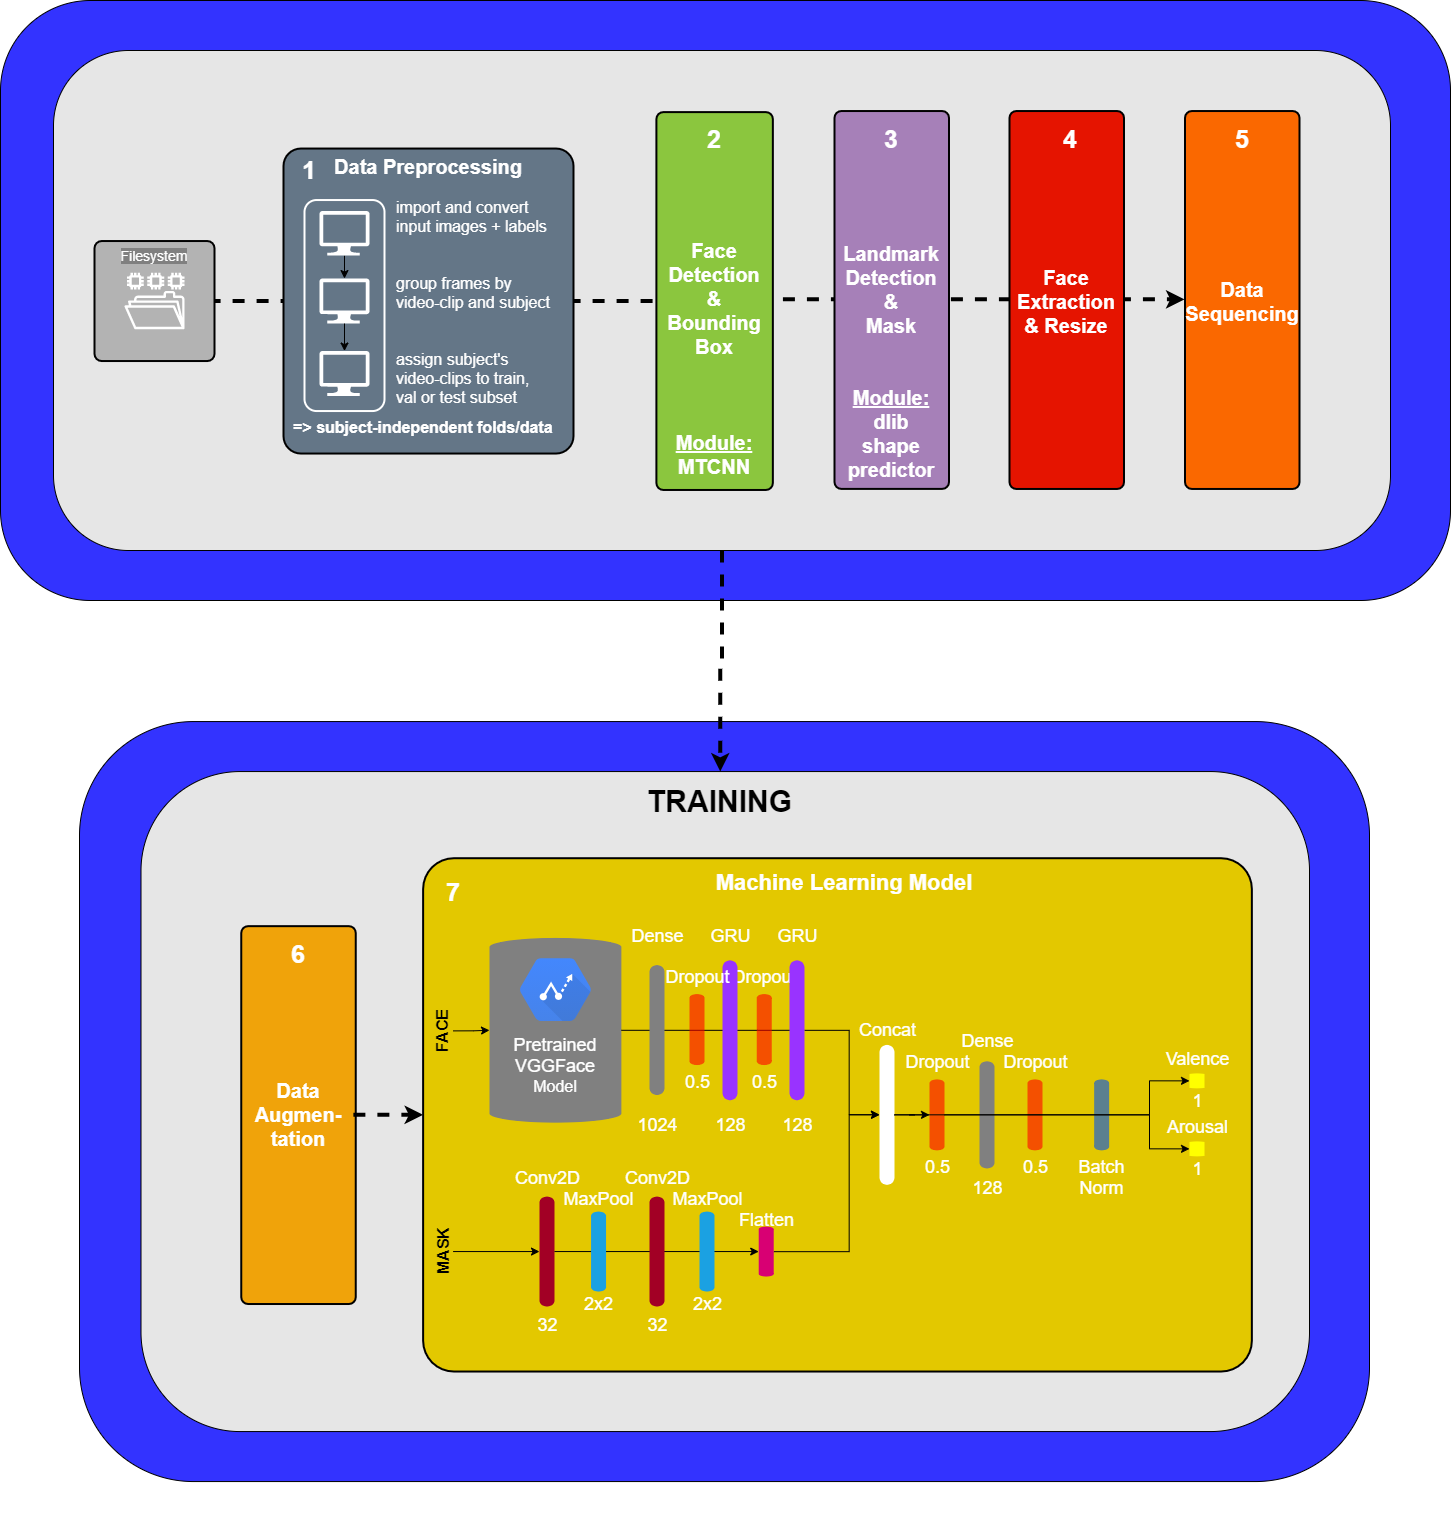
\includegraphics[width=1.1\textwidth]{Figures/EmotionRecognitionInTheWild-RNN_Pipeline.png}}
  \caption{The emotion recognition pipeline in this Master's thesis requires seven essential steps}
  \label{fig:MachineLearningModelMethods}
  \end{center}
\end{figure}

Figure \ref{fig:MachineLearningModelMethods} illustrates the emotion recognition pipeline in this Master's thesis that consists of two stages. The first stage is separate as it is performed initially on the whole dataset, while the methods in the training stage are applied on a per batch basis during the optimization of the neural network.
\newline\newline
First, video frames and their labels were imported, grouped by subject and assigned to either the training, validation or testing subset. This ensured the creation of subject-independent folds/data. Second, for each frame the face was detected and a bounding box was determined using a pre-trained network optimized for face detection, namely MTCNN \citep{Zhang:2016:MTCCN}.
\newline\newline
Third, landmarks were detected based on the previously determined bounding box. These landmarks were then saved as a mask in a 2-dimensional image for the usage as an input for machine learning model. Fourth, the face was extracted from the image by cropping it along the borders of the bounding box. The resulting extract was then resized to a 224x224 format. Fifth, the extracted face were put into a sequence of 45 frames for each video-clip.
\newline\newline
Sixth, data augmentation was applied in order to significantly increase the diversity of the images in the underlying dataset. Seventh, data was passed into the machine learning model, consisting of a the pre-trained VGGFace \citep{Cao:2018:VGGFace2} neural network that was extended with a Recurrent Neural Network (RNN) as a custom classifier. In this way, the output features of the VGGFace network for each frame in a video-clip are combined and fed into the RNN which then learns  tempo-spatial aspects of a video-clip. The VGGFace network will be discussed in more details in section \ref{sec:Training&Regularization}.

%%%%%%%%%%%%%%%%%%%%%%%
\section{Data preprocessing}
The very first step in the proposed pipeline, as shown in figure \ref{fig:MachineLearningModelMethods}, is data preprocessing. Here, the input images/frames were imported and converted into the right format. Their corresponding labels, originally in the scale of -10 to +10, were re-scaled to -1 to +1 in order to fit the chosen 'tanh' activation function of the machine learning model.
\newline\newline
Samples of the input images and their corresponding output labels are shown in figure \ref{fig:MethodologyPreprocess}. Output labels consist of valence (=expression of how positive or negative an emotion is) and arousal (=expression of how strong or weak an emotion is).

\begin{figure}[ht]
  \centering
  \subfloat[V: 0.0, A: +0.5]{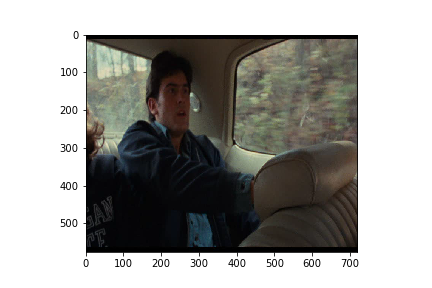
\includegraphics[width=0.5\textwidth]{Figures/001/001_1_00000.png}}
  \hfill
  \subfloat[V: 0.0, A: +0.5]{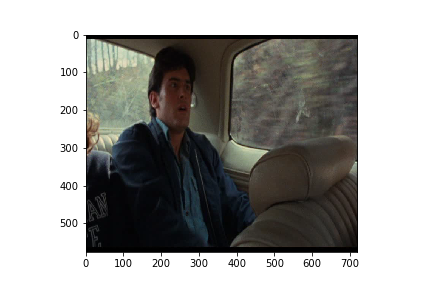
\includegraphics[width=0.5\textwidth]{Figures/001/001_1_00011.png}}
  \hfill
  \subfloat[V: +0.2, A: +0.3]{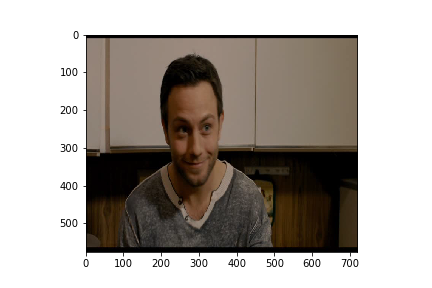
\includegraphics[width=0.5\textwidth]{Figures/002/002_1_00000.png}}
  \hfill
  \subfloat[V: +0.2, A: +0.4]{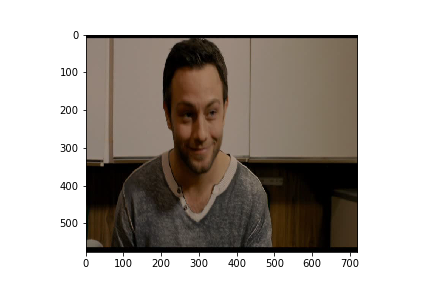
\includegraphics[width=0.5\textwidth]{Figures/002/002_1_00011.png}}
  \hfill
  \subfloat[V: -0.5, A: +0.3]{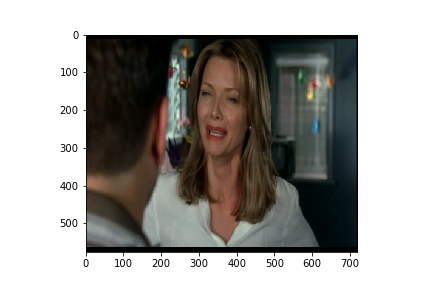
\includegraphics[width=0.5\textwidth]{Figures/576/576_1_00000.png}}
  \hfill
  \subfloat[V: -0.6, A: +0.3]{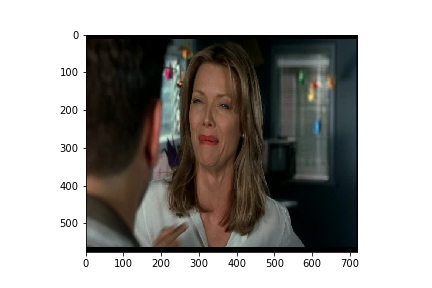
\includegraphics[width=0.5\textwidth]{Figures/576/576_1_00011.png}}
  \caption{Sample frames from the AFEW-VA dataset \citep{Kossaifi:2017:AFEW-VADatabase} and their corresponding labels representing the valence (V) and arousal (A) as values between -1 and +1.}
  \label{fig:MethodologyPreprocess}
\end{figure}

Furthermore, for the later following sequencing step, the frames were already grouped by video-clips and by subject. With this, a subject's video-clips could be assigned to either the training, validation or testing subset in a subject-independent manner. This results in the whole dataset being split into 80\% for training, 10\% for validation and 10\% for testing.

\section{Face Detection} \label{sec:FaceDetection}
The second step in the proposed pipeline involves detecting the faces in each frame of the video. This is valuable in order to determine the face's bounding box which is need in a further stage of the pipeline for the detection of landmarks and the cropping of the image. To achieve this, the Multi-Task Cascaded Convolutional Neural Network (MTCNN) by \citet{Zhang:2016:MTCCN} was used.
\newline\newline
MTCNN is a pre-trained neural network optimized for the tasks of simultaneous face detection, face alignment, bounding boxing and landmark detection \citep{Brownlee:2019:VggFace2HowToFaceRec}. This makes it ideal for the purpose of determining the face's bounding box in the face of the video frames. In figure \ref{fig:MethodologyBoundingBox} successful examples of the application of the MTCNN algorithm are shown by overlaying the bounding box on the image.

\begin{figure}[ht]
  \centering
  \subfloat[V: 0.0, A: +0.5]{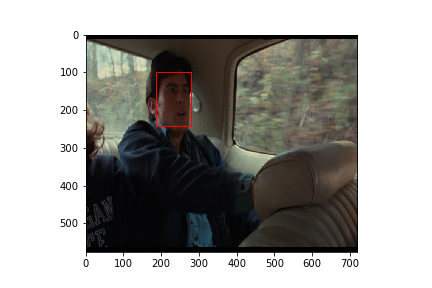
\includegraphics[width=0.5\textwidth]{Figures/001/001_2_00000.png}}
  \hfill
  \subfloat[V: 0.0, A: +0.5]{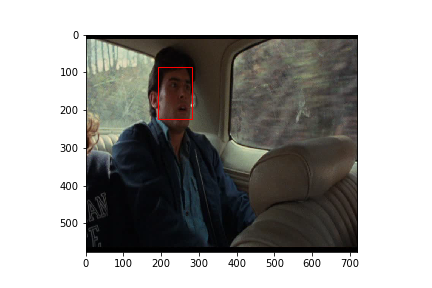
\includegraphics[width=0.5\textwidth]{Figures/001/001_2_00011.png}}
  \hfill
  \subfloat[V: +0.2, A: +0.3]{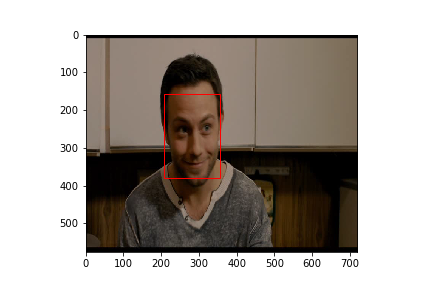
\includegraphics[width=0.5\textwidth]{Figures/002/002_2_00000.png}}
  \hfill
  \subfloat[V: +0.2, A: +0.4]{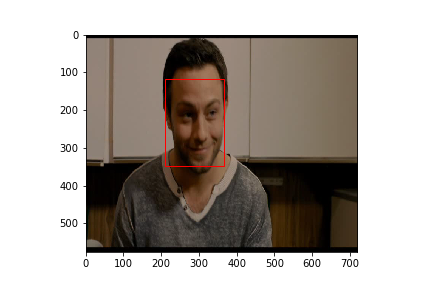
\includegraphics[width=0.5\textwidth]{Figures/002/002_2_00011.png}}
  \hfill
  \subfloat[V: -0.5, A: +0.3]{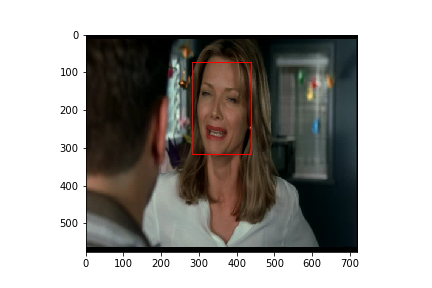
\includegraphics[width=0.5\textwidth]{Figures/576/576_2_00000.png}}
  \hfill
  \subfloat[V: -0.6, A: +0.3]{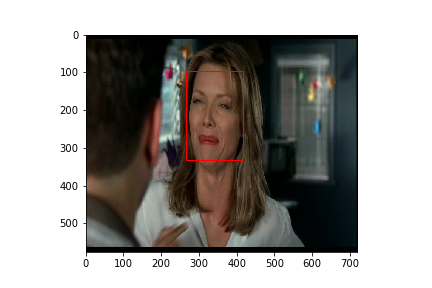
\includegraphics[width=0.5\textwidth]{Figures/576/576_2_00011.png}}
  \caption{Visualization of the bounding box detected by the MTCNN face detection module \citep{Zhang:2016:MTCCN} and their corresponding labels representing the valence (V) and arousal (A) as values between -1 and +1.}
  \label{fig:MethodologyBoundingBox}
\end{figure}



\section{Landmark Detection}
The third step in the proposed pipeline involves the detection of facial landmarks in each frame. This is a preliminary step for the generation of two-dimensional mask, as it is based on the coordinates of the landmark points.
\newline\newline
This was done using a 'Face Landmark Detection' algorithm based on the work done by \citet{Kazemi:2014:ShapePredictor}. The algorithm is based on an ensemble of regression trees which successively aligns the constructed shape model to the specific features of the the face at hand.
\newline\newline
The input of the algorithm consists of the frame, as well as coordinates of the face's bounding box. The algorithm's output is made up of 68 facial landmarks of a person's face. Examples of this successful operation are shown in figure \ref{fig:MethodologyLandmarks} by overlaying the landmark dots on the input image.
\citep{Datahacker:2020:DlibFacialLandmarks}

\begin{figure}[ht]
  \centering
  \subfloat[V: 0.0, A: +0.5]{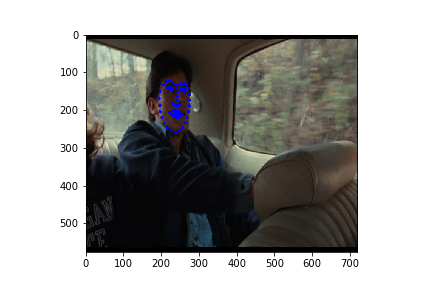
\includegraphics[width=0.5\textwidth]{Figures/001/001_3_00000.png}}
  \hfill
  \subfloat[V: 0.0, A: +0.5]{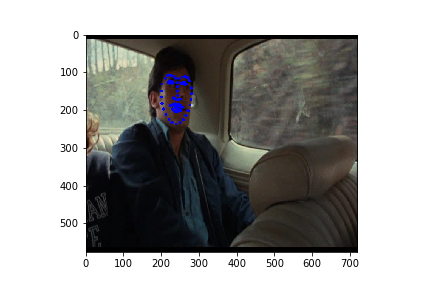
\includegraphics[width=0.5\textwidth]{Figures/001/001_3_00011.png}}
  \hfill
  \subfloat[V: +0.2, A: +0.3]{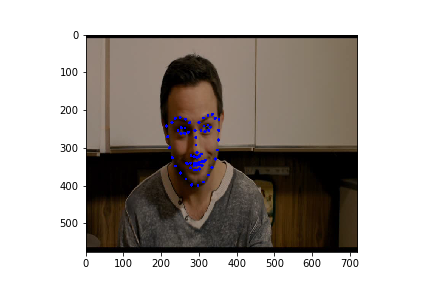
\includegraphics[width=0.5\textwidth]{Figures/002/002_3_00000.png}}
  \hfill
  \subfloat[V: +0.2, A: +0.4]{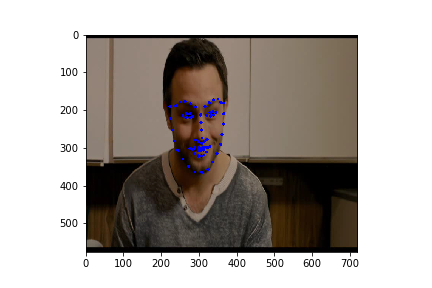
\includegraphics[width=0.5\textwidth]{Figures/002/002_3_00011.png}}
  \hfill
  \subfloat[V: -0.5, A: +0.3]{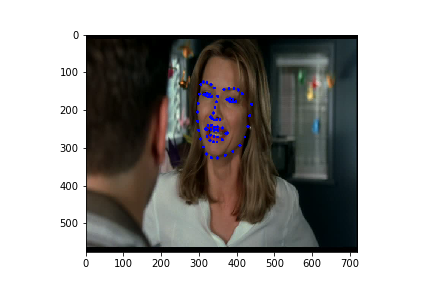
\includegraphics[width=0.5\textwidth]{Figures/576/576_3_00000.png}}
  \hfill
  \subfloat[V: -0.6, A: +0.3]{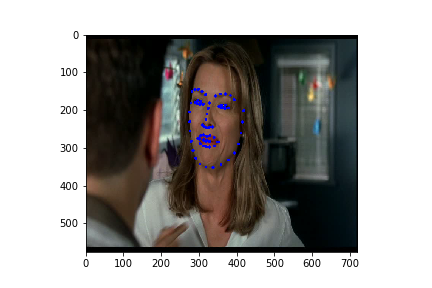
\includegraphics[width=0.5\textwidth]{Figures/576/576_3_00011.png}}
  \caption{Visualization of the landmarks detected by the pre-trained 'Face Landmark Detection' algorithm \citep{Kazemi:2014:ShapePredictor} and their corresponding labels representing the valence (V) and arousal (A) as values between -1 and +1.}
  \label{fig:MethodologyLandmarks}
\end{figure}

These landmarks were then used to generate a two-dimensional mask. This mask can then be fed as a separate input, next to the image, into the neural network. Such a musk would then enable the network to learn differentiate the importance of areas in an input image. Results of the generated landmark mask can be seen in figure \ref{fig:MethodologyMask}.

\begin{figure}[ht]
  \centering
  \subfloat[V: 0.0, A: +0.5]{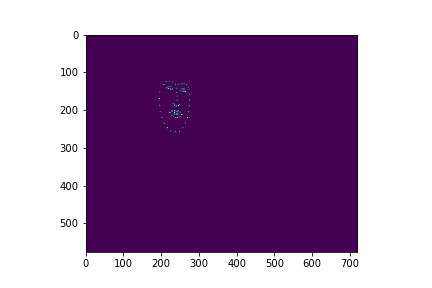
\includegraphics[width=0.5\textwidth]{Figures/001/001_4_00000.png}}
  \hfill
  \subfloat[V: 0.0, A: +0.5]{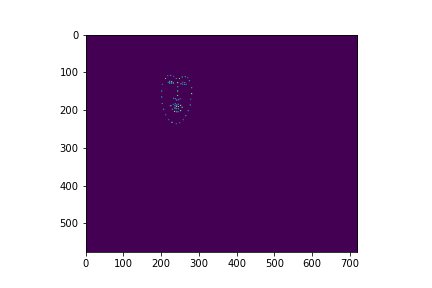
\includegraphics[width=0.5\textwidth]{Figures/001/001_4_00011.png}}
  \hfill
  \subfloat[V: +0.2, A: +0.3]{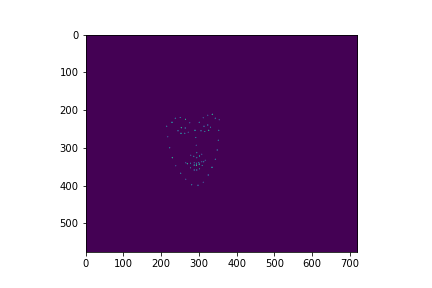
\includegraphics[width=0.5\textwidth]{Figures/002/002_4_00000.png}}
  \hfill
  \subfloat[V: +0.2, A: +0.4]{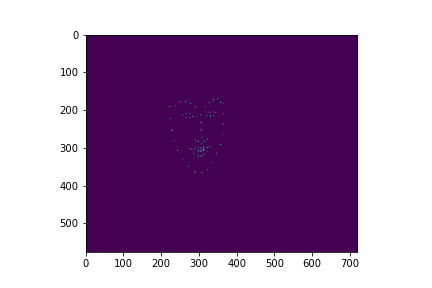
\includegraphics[width=0.5\textwidth]{Figures/002/002_4_00011.png}}
  \hfill
  \subfloat[V: -0.5, A: +0.3]{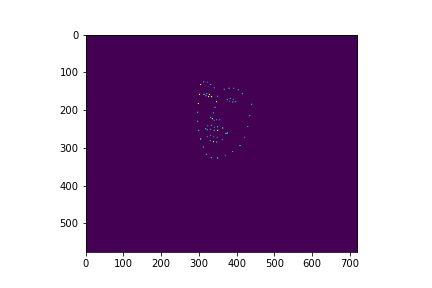
\includegraphics[width=0.5\textwidth]{Figures/576/576_4_00000.png}}
  \hfill
  \subfloat[V: -0.6, A: +0.3]{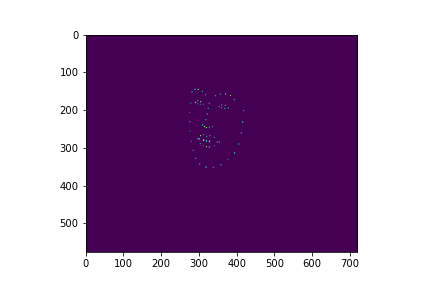
\includegraphics[width=0.5\textwidth]{Figures/576/576_4_00011.png}}
  \caption{Visualization of the generated mask based on detected landmark points and their corresponding labels representing the valence (V) and arousal (A) as values between -1 and +1.}
  \label{fig:MethodologyMask}
\end{figure}


%%%%%%%%%%%%%%%%%%%%%%%%%%%%%%%%%%%%%%%%%%%%%%%%%%%%%
\section{Face Extraction}
The fourth step in the proposed pipeline involves the extraction of the face from the original input image, as well as the same extraction performed on the mask. This is valuable as it removes unimportant information/features of the image's background which could otherwise negatively affect the learning process.
\newline\newline
This step was conducted by simply cropping the face along the border lines of the face's bounding box. The output is again a image with a dimensions of 224x224 pixels that displays the inner area of the bounding box, namely the person's face. Example outputs are illustrated in figure \ref{fig:MethodologyExtraction}. At the same time, also the mask had to be cropped in along the same border lines of the face's bounding box. Results of this are presented in figure \ref{fig:MethodologyExtractionMask}.

\begin{figure}[ht]
  \centering
  \subfloat[V: 0.0, A: +0.5]{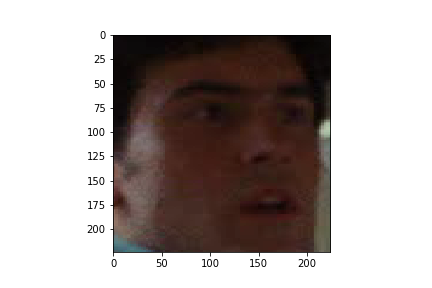
\includegraphics[width=0.5\textwidth]{Figures/001/001_5_00000.png}}
  \hfill
  \subfloat[V: 0.0, A: +0.5]{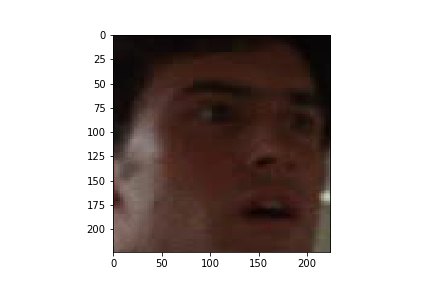
\includegraphics[width=0.5\textwidth]{Figures/001/001_5_00011.png}}
  \hfill
  \subfloat[V: +0.2, A: +0.3]{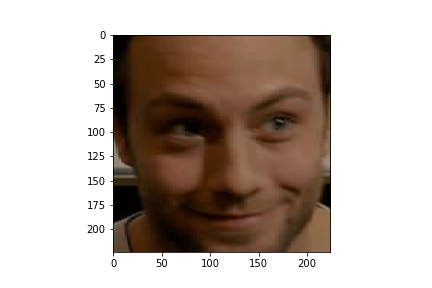
\includegraphics[width=0.5\textwidth]{Figures/002/002_5_00000.png}}
  \hfill
  \subfloat[V: +0.2, A: +0.4]{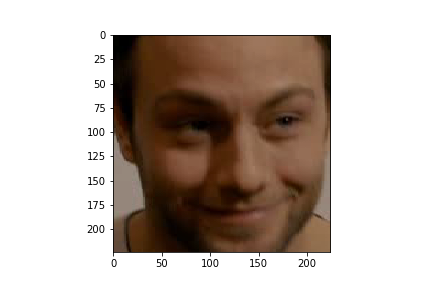
\includegraphics[width=0.5\textwidth]{Figures/002/002_5_00011.png}}
  \hfill
  \subfloat[V: -0.5, A: +0.3]{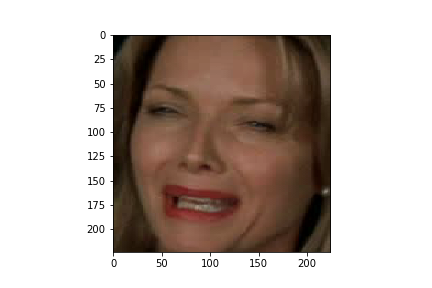
\includegraphics[width=0.5\textwidth]{Figures/576/576_5_00000.png}}
  \hfill
  \subfloat[V: -0.6, A: +0.3]{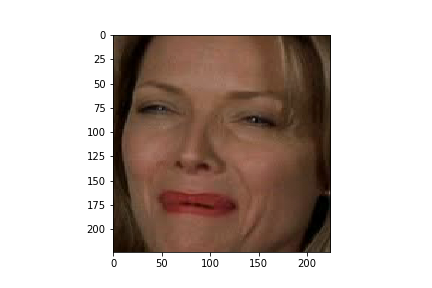
\includegraphics[width=0.5\textwidth]{Figures/576/576_5_00011.png}}
  \caption{Visualization of the extracted face and their corresponding labels representing the valence (V) and arousal (A) as values between -1 and +1.}
  \label{fig:MethodologyExtraction}
\end{figure}

\begin{figure}[ht]
  \centering
  \subfloat[V: 0.0, A: +0.5]{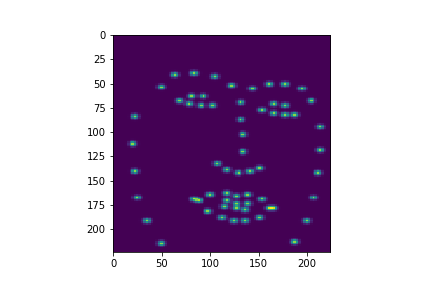
\includegraphics[width=0.5\textwidth]{Figures/001/001_5_2_00000.png}}
  \hfill
  \subfloat[V: 0.0, A: +0.5]{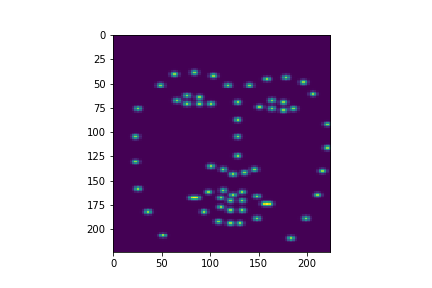
\includegraphics[width=0.5\textwidth]{Figures/001/001_5_2_00011.png}}
  \hfill
  \subfloat[V: +0.2, A: +0.3]{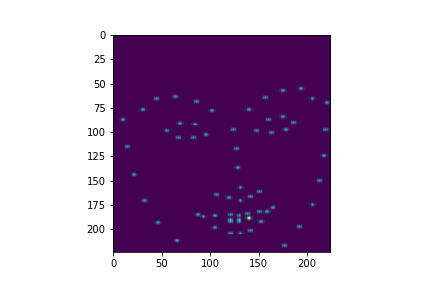
\includegraphics[width=0.5\textwidth]{Figures/002/002_5_2_00000.png}}
  \hfill
  \subfloat[V: +0.2, A: +0.4]{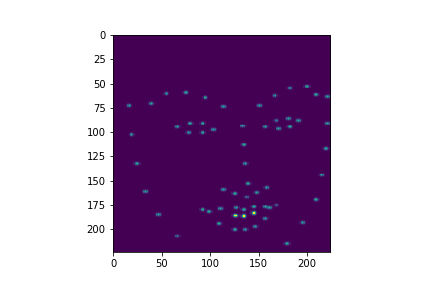
\includegraphics[width=0.5\textwidth]{Figures/002/002_5_2_00011.png}}
  \hfill
  \subfloat[V: -0.5, A: +0.3]{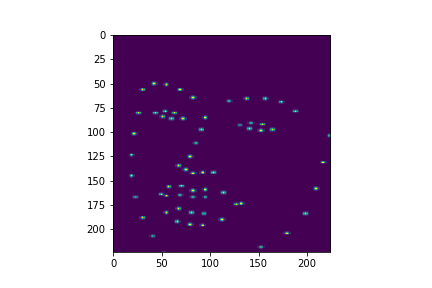
\includegraphics[width=0.5\textwidth]{Figures/576/576_5_2_00000.png}}
  \hfill
  \subfloat[V: -0.6, A: +0.3]{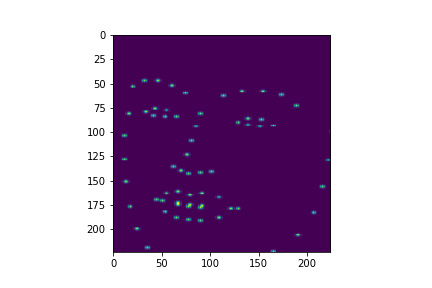
\includegraphics[width=0.5\textwidth]{Figures/576/576_5_2_00011.png}}
  \caption{Visualization of the extracted mask and their corresponding labels representing the valence (V) and arousal (A) as values between -1 and +1.}
  \label{fig:MethodologyExtractionMask}
\end{figure}

%%%%%%%%%%%%%
\section{Data Sequencing}
In the fifth step, video-clips out of their respective subset (train, validation or test) are further processed in a way that each clip contains exactly 45 frames. The number of 45 frames was chosen slightly below the median number of frames per video (= 45.5) across the whole AFEW-VA dataset.
\newline\newline
Achieving this exact number of frames per video-clip, required frames to be either removed or added. This was done by duplicating or removing frames at a regular interval depending on the ratio between the actual number of frames per video-clip and the desired sequence length of 45. At the same time this action was also applied to the face's corresponding mask.
\newline\newline
Overall, the sequencing step resulted in an reduction of the dataset size from around 30.050 frames (average number of 50.1 frames + median number of 45.5 frames per video-clips) to 27.000 frames (average \& median number of 45 frames per video-clip). However, there are another 27.000 images saved as corresponding masks for the extracted faces.

%%%%%%%%%%%%%
\section{Data Augmentation}
The sixth step of the proposed pipeline involves the augmentation of the input images in order to increase its variety before feeding them into the neural network. In that way, the model will see more slightly different images and increases its ability to better generalize from training data. Even though data augmentation was applied during training to both, the face and it's corresponding mask, figure \ref{fig:MethodologyDataAugmentation} only presents examples from augmented faces.

\begin{figure}[ht]
  \centering
  \subfloat[V: 0.0, A: +0.5]{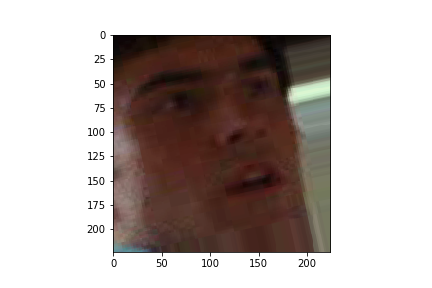
\includegraphics[width=0.5\textwidth]{Figures/001/001_6_00000.png}}
  \hfill
  \subfloat[V: 0.0, A: +0.5]{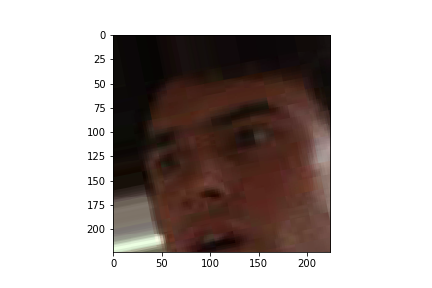
\includegraphics[width=0.5\textwidth]{Figures/001/001_6_00011.png}}
  \hfill
  \subfloat[V: +0.2, A: +0.3]{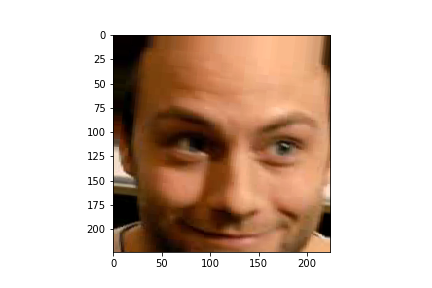
\includegraphics[width=0.5\textwidth]{Figures/002/002_6_00000.png}}
  \hfill
  \subfloat[V: +0.2, A: +0.4]{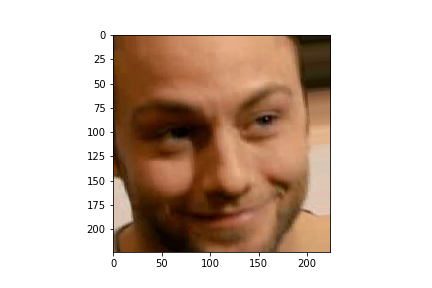
\includegraphics[width=0.5\textwidth]{Figures/002/002_6_00011.png}}
  \hfill
  \subfloat[V: -0.5, A: +0.3]{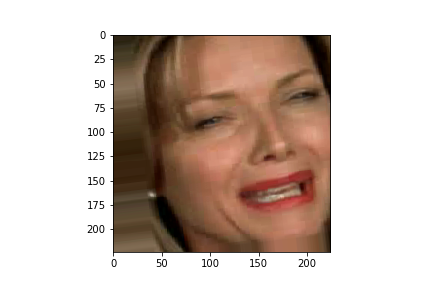
\includegraphics[width=0.5\textwidth]{Figures/576/576_6_00000.png}}
  \hfill
  \subfloat[V: -0.6, A: +0.3]{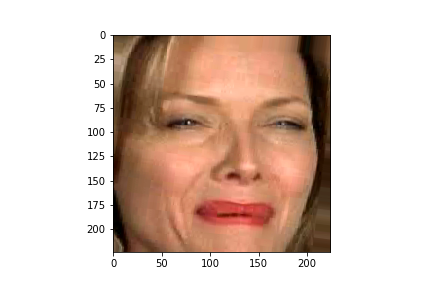
\includegraphics[width=0.5\textwidth]{Figures/576/576_6_00011.png}}
  \caption{Visualization of augmented faces and their corresponding labels representing the valence (V) and arousal (A) as values between -1 and +1.}
  \label{fig:MethodologyDataAugmentation}
\end{figure}


%%%%%%%%%%%%%%%%%%%%%%%%%%%%%%%%%%%%%%%%%%%%%%%%%%%%%
\section{Machine Learning Model for Emotion Recognition}
In the final step of the proposed pipeline, the augmented frames are fed into the machine learning model for training on the emotion recognition challenge. The model's architecture, consisting of the pre-trained VGGFace model \citep{Cao:2018:VGGFace2} and a custom classifier, can be seen in figure \ref{fig:MachineLearningModel}.
\newline\newline
The VGGFace model architecture, is based on the famous ResNet-50 convolutional neural network which the authors \citet{Cao:2018:VGGFace2} pre-trained on a large-scale face dataset, named VGGFace2. The dataset contains about 3.31 million images of 9131 subjects and poses, which provided a wide variety of poses, ages, etc. When the VGGFace2 paper, written by \citet{Cao:2018:VGGFace2}, was published in \citeyear{Cao:2018:VGGFace2}, it exceeded the performance of previous state-of-the-art by a large margin \citep{Cao:2018:VGGFace2}.

\begin{figure}[H]
  \begin{center}
  \makebox[\textwidth][c]{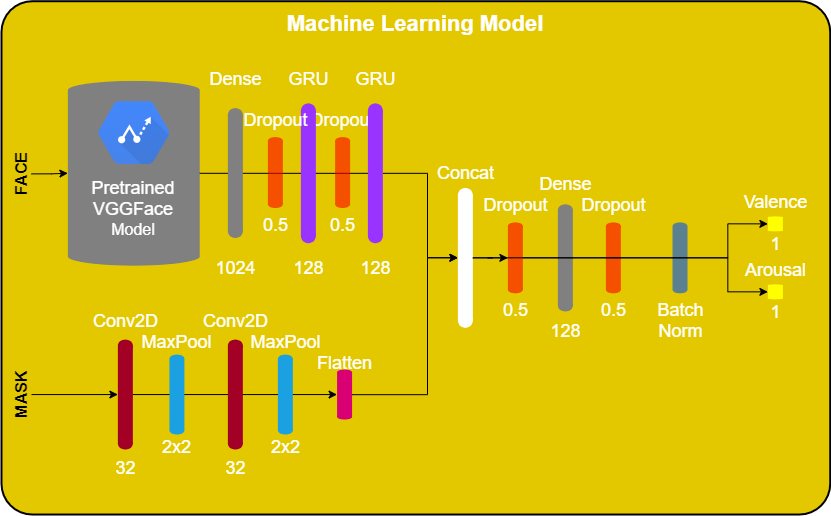
\includegraphics[width=0.8\textwidth]{Figures/MachineLearningModel.png}}
  \caption{The machine learning model consists of a pre-trained VGGFace network and a custom added RNN. The face's masks is processed through a different Convolutional Neural Network. Both outputs are connected and contribute twoard the recognition of valence and arousal.}
  \label{fig:MachineLearningModel}
  \end{center}
\end{figure}

The utilization of a pre-trained neural network is often referred to as transfer learning. \citet{Pedro:2018:TransferLearning} supports that instead of training the model from scratch, transfer learning allows to start the training process from patterns that have already been learned by solving a different problem.
\newline\newline
In this work, a version of the VGGFace model that was pre-trained on the VGGFace2 dataset \citep{Cao:2018:VGGFace2} for the task of face identification has been used. The pre-trained model was then further fine-tuned on the AFEW-VA dataset \citep{Kossaifi:2017:AFEW-VADatabase}. In this way, learnt patterns about facial features from the face identification task were used to kick-start the learning for emotion recognition from there. 
\newline\newline
A noteworthy architectural change was the removal of the last fully-connected layers at the end of VGGFace. For this work, these layers were replaced with another classifier in order to learn the correlation between facial features and their target labels for the emotion recognition task. The architecture of the newly added classifier, as shown in figure \ref{fig:MachineLearningModel}, includes a Recurrent Neural Network (RNN) for capturing tempo-spatial information.